%----------------------------------------------------------------------------------------
%	PACKAGES AND THEMES
%----------------------------------------------------------------------------------------
\documentclass[aspectratio=169,xcolor=dvipsnames, t]{beamer}
\usepackage{fontspec} % Allows using custom font. MUST be before loading the theme!
\usetheme{SimplePlusAIC}
\usepackage{hyperref}
\usepackage{graphicx} % Allows including images
\usepackage{booktabs} % Allows the use of \toprule, \midrule and  \bottomrule in tables
\usepackage{svg} %allows using svg figures
\usepackage{tikz}
\usepackage{makecell}
\usepackage{wrapfig}
% ADD YOUR PACKAGES BELOW

%----------------------------------------------------------------------------------------
%	TITLE PAGE CONFIGURATION
%----------------------------------------------------------------------------------------

\title[short title]{Zadanie 2 LaTeX } % The short title appears at the bottom of every slide, the full title is only on the title page
\subtitle{podtytuł}

\author[autor]{Tomasz Raczunas}
\institute[UG]{Uniwersytet Gdański \newline Wydział Informatyki}
% Your institution as it will appear on the bottom of every slide, maybe shorthand to save space


\date{\today} % Date, can be changed to a custom date
%----------------------------------------------------------------------------------------
%	PRESENTATION SLIDES
%----------------------------------------------------------------------------------------

\begin{document}

\maketitlepage

%------------------------------------------------

\begin{frame}{Lista wypunktowana i Lista ponumerowana}
\pause
    \begin{itemize}
        \item Lorem ipsum dolor sit amet, consectetur adipiscing elit
        \item Aliquam blandit faucibus nisi, sit amet dapibus enim tempus eu
        \item Nulla commodo, erat quis gravida posuere, elit lacus lobortis est, quis porttitor odio mauris at libero
        \item Nam cursus est eget velit posuere pellentesque
    \end{itemize}
\
\pause
%------------------------------------------------
% Lists

    \begin{enumerate}
        \item Lorem ipsum dolor sit amet, consectetur adipiscing elit
        \item Aliquam blandit faucibus nisi, sit amet dapibus enim tempus eu
        \item Vestibulum faucibus velit a augue condimentum quis convallis nulla gravida
        \item Nam cursus est eget velit posuere pellentesque
    \end{enumerate}
\end{frame}


%------------------------------------------------
% Table
\begin{frame}{TABELA}
    \begin{table}
        \begin{tabular}{l l l}
            \toprule
            \textbf{Temat 1} & \textbf{Temat 2} & \textbf{Temat 3} \\
            \midrule
            Tekst 1         & Tekst 2           & Tekst 3               \\
            Tekst 1         & Tekst 2           & Tekst 3               \\
            Tekst 1         & Tekst 2           & Tekst 3               \\
            Tekst 1         & Tekst 2           & Tekst 3               \\
            \bottomrule
        \end{tabular}
        \caption{Przykładowa tabela}
        \label{tabela}
    \end{table}
\end{frame}

%------------------------------------------------

\begin{frame}{ANDROID}
    \begin{wrapfigure}{r}{0.4\textwidth}
    \centering
        
\includegraphics[width=0.5\linewidth]{android.png}
    \caption{Android logo}
    \label{fig:android}
\end{wrapfigure}

Android – system operacyjny z jądrem bazującym na Linuksie dla urządzeń mobilnych takich jak telefony komórkowe, smartfony, tablety i netbooki. W 2013 roku był najpopularniejszym systemem mobilnym na świecie. Główna część systemu jest otwartym oraz wolnym oprogramowaniem.

\end{frame}

%------------------------------------------------

\begin{frame}{MICROSOFT}
    \begin{wrapfigure}{r}{0.4\textwidth}
    \centering
    
\includegraphics[width=0.5\linewidth]{microsoft.png}
    \caption{Microsoft logo}
    \label{fig:Microsoft}
\end{wrapfigure}

Microsoft Corporation \footnote{Duża korporacja} – amerykańskie przedsiębiorstwo informatyczne. Najbardziej znane jako producent systemów operacyjnych MS-DOS, Microsoft Windows i oprogramowania biurowego Microsoft Office. Spółka publiczna z siedzibą w Redmond w stanie Waszyngton. Założona w 1975 roku przez Billa Gatesa i Paula Allena.



\end{frame}

%------------------------------------------------
\begin{frame}{NVIDIA}
    \begin{wrapfigure}{r}{0.4\textwidth}
    \centering
    
\includegraphics[width=0.5\linewidth]{nvidia.png}
    \caption{Nvidia logo}
    \label{fig:nvidia}
\end{wrapfigure}

NVIDIA Corporation – amerykańskie przedsiębiorstwo komputerowe będące jednym z największych na świecie producentów procesorów graficznych i innych układów scalonych przeznaczonych na rynek komputerowy. NVIDIA jest także głównym dostawcą kart graficznych dla komputerów osobistych ze swoją standardową serią GeForce

\end{frame}
%------------------------------------------------
\begin{frame}{AMD}
    \begin{wrapfigure}{r}{0.4\textwidth}
    \centering
    
\includegraphics[width=0.5\linewidth]{amd.png}
    \caption{AMD logo}
    \label{fig:AMD}
\end{wrapfigure}

Advanced Micro Devices, Inc., AMD – amerykańskie przedsiębiorstwo produkujące elektronikę (głównie układy scalone) dla użytkowników domowych i firm z siedzibą w Santa Clara[2][3]. Do głównych produktów AMD należą mikroprocesory, chipsety do płyt głównych, systemy wbudowane, FPGA oraz procesory graficzne dla serwerów, stacji roboczych i komputerów PC.
\end{frame}
%------------------------------------------------
\begin{frame}{USB}
    \begin{wrapfigure}{r}{0.4\textwidth}
    \centering
    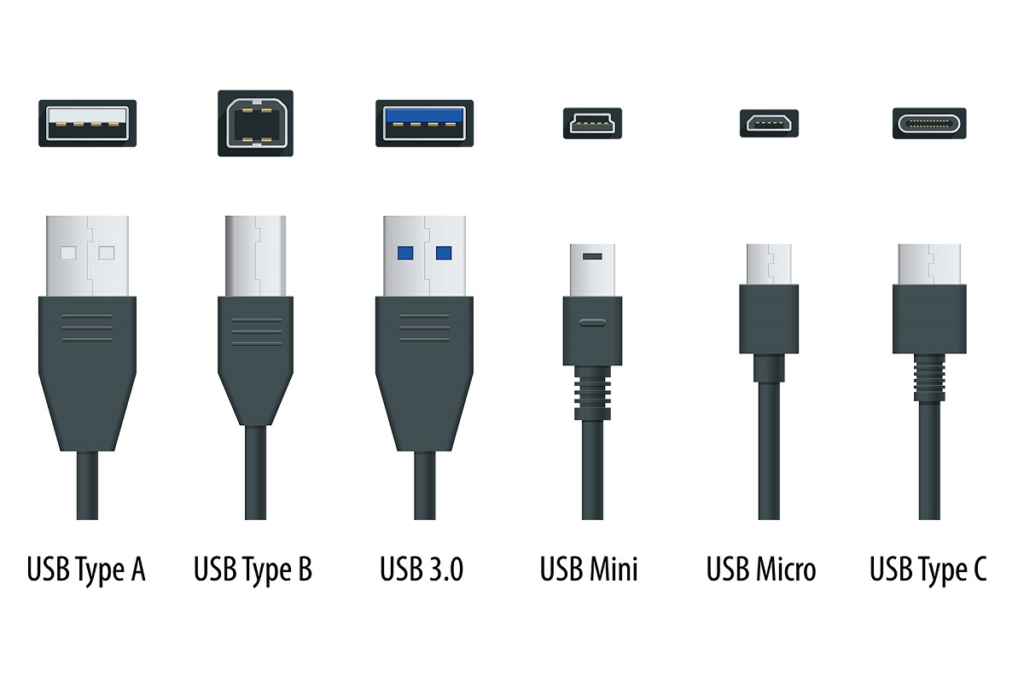
\includegraphics[width=0.9\linewidth]{usb.png}
    \caption{Rodzaje usb}
    \label{fig:usb}
\end{wrapfigure}
USB, uniwersalna magistrala szeregowa – komputerowe złącze komunikacyjne zastępujące stare porty szeregowe i porty równoległe. Zostało opracowane przez firmy Microsoft, Intel, Compaq, IBM i DEC. Port USB jest uniwersalny w tym sensie, że można go wykorzystać do podłączenia do komputera wielu różnych urządzeń.
\end{frame}




%------------------------------------------------
\begin{frame}[fragile] 
    \frametitle{Odwołania}
    Odwołanie do tabeli:
    
    \ref{tabela} Do tabeli
\hfill \break

    Odwołania do bibliografii:
    
    \cite{book1} Potop
    
    \cite{book2} Inna książka
    
\hfill \break   
    Odwołania do obrazków:
    
    \ref{fig:android} Do logo Android
       
    \ref{fig:Microsoft} Do logo Microsoft
    
    \ref{fig:nvidia} Do logo Nvidia

    \ref{fig:AMD} Do logo AMD
    
    \ref{fig:usb} Do porównania USB
\end{frame}

%------------------------------------------------
% Refenrenced
\begin{frame}{Bibliografia}
    \footnotesize{
    \begin{thebibliography}{5}
        \bibitem{book1}
        Henryk Sienkiewicz,
        \emph{Potop},
        PWN,
        1886
        
        \bibitem{book2}
        Jakaś tam inna książka z bibliografii
        
        \bibitem{book3}
        Jakaś tam kolejna książka z bibliografii
        
    \end{thebibliography}
    }
\end{frame}


\finalpagetext{Dziękuję za uwagę}
\makefinalpage
%----------------------------------------------------------------------------------------
\end{document}
